\documentclass[a4paper,12pt]{article}

\usepackage[utf8]{inputenc}
\usepackage[T1]{fontenc}
\usepackage[italian]{babel}
\usepackage{lmodern}
\usepackage{geometry}
\usepackage{graphicx}
\usepackage{booktabs}
\usepackage{tabularx}
\usepackage{amsmath}
\usepackage{float}
\usepackage{hyperref}
\usepackage{setspace}
\usepackage{enumitem}

\geometry{margin=2.5cm}
\setstretch{1.1}
\graphicspath{{figures/}}
\hypersetup{
    colorlinks=true,
    linkcolor=black,
    urlcolor=blue,
    citecolor=black
}

\title{\textbf{Profilazione della coerenza della qualit\`a dell'aria urbana mediante Relaxed Functional Dependencies}}
\author{
    Nome Cognome \\
    Matricola: XXXXXXX \\
    Corso: XXXXXXX
}
\date{\today}

\begin{document}

\maketitle

\begin{abstract}
Questo report presenta un'analisi riproducibile della qualit\`a dell'aria urbana formulata come caso di studio per un \textit{Urban Digital Twin} in senso concettuale. Il dataset impiegato \`e un sottoinsieme del \textit{Beijing Multi-Site Air Quality Data Set}, limitato alle stazioni \textit{Aotizhongxin} e \textit{Changping} nel periodo settembre--dicembre 2013. L'obiettivo \`e valutare se relazioni approssimate tra variabili ambientali possano essere descritte tramite \textit{Relaxed Functional Dependencies} (RFDs). Dopo preprocessing e profiling, sono state validate regole candidate e condotta una scoperta leggera su un campione bilanciato di 1500 righe. Il dataset finale contiene 5426 osservazioni e 11 variabili. La regola candidata pi\`u solida risulta \texttt{station, PM2.5 $\rightarrow$ PM10}, con supporto 0.073 e confidenza 0.466 in configurazione \textit{medium}. Nessuna regola scoperta automaticamente soddisfa simultaneamente i vincoli finali di supporto e confidenza. Il risultato suggerisce che le RFD sono utili soprattutto come strumento di profilazione della coerenza e analisi delle violazioni, non come base per inferenze causali.
\end{abstract}

\section{Introduzione}
Il paradigma di \textit{Urban Digital Twin} viene spesso associato a rappresentazioni digitali integrate del sistema urbano. In questo progetto il termine \`e usato in modo volutamente minimo: non si costruisce una piattaforma 3D o un'infrastruttura real-time, ma un supporto analitico riproducibile per lo studio di coerenze e anomalie in dati ambientali storici.

L'approccio adottato si basa sulle \textit{Relaxed Functional Dependencies}. Una RFD estende la dipendenza funzionale classica sostituendo l'uguaglianza esatta con la similarit\`a: se due tuple sono sufficientemente simili sul lato sinistro, ci si attende che rimangano simili anche sul lato destro. In un dominio come la qualit\`a dell'aria, questa impostazione \`e preferibile a regole deterministiche rigide, perch\'e i fenomeni osservati sono variabili, rumorosi e influenzati da fattori non misurati.

L'obiettivo del lavoro \`e duplice: da un lato descrivere in modo sintetico il comportamento del dataset, dall'altro verificare se emergano regolarit\`a approssimate interpretabili tra inquinanti e covariate meteorologiche.

Pi\`u precisamente, il progetto si propone di:
\begin{enumerate}[leftmargin=1.2cm]
    \item costruire un dataset pulito e documentato a partire da dati grezzi di monitoraggio ambientale;
    \item produrre un profiling descrittivo utile a contestualizzare le successive verifiche di coerenza;
    \item validare un piccolo insieme di regole RFD motivate da intuizioni ambientali plausibili;
    \item confrontare il comportamento delle regole al variare delle soglie di similarit\`a e tra stazioni diverse;
    \item discutere le violazioni come possibili segnali di eterogeneit\`a, rumore o fattori non osservati.
\end{enumerate}

\section{Dati e preprocessing}
Il dataset di partenza \`e il \textit{Beijing Multi-Site Air Quality Data Set} della UCI Machine Learning Repository \cite{uci}. Per contenere il costo degli esperimenti pairwise sono state selezionate soltanto due stazioni, \texttt{Aotizhongxin} e \texttt{Changping}, e una finestra temporale compresa tra il 1 settembre 2013 e il 31 dicembre 2013. La finestra settembre--novembre produceva 3996 righe complete; l'inclusione di dicembre porta il dataset a 5426 righe, valore pi\`u adatto allo scopo del progetto.

Le variabili finali sono:
\texttt{datetime}, \texttt{station}, \texttt{hour}, \texttt{PM2.5}, \texttt{PM10}, \texttt{NO2}, \texttt{O3}, \texttt{TEMP}, \texttt{DEWP}, \texttt{WSPM}, \texttt{time\_slot}. La variabile \texttt{time\_slot} aggrega l'ora in quattro classi: \texttt{night}, \texttt{morning}, \texttt{afternoon}, \texttt{evening}. La gestione dei mancanti \`e stata intenzionalmente semplice: calcolo del riepilogo, eliminazione delle righe incomplete sulle colonne finali e nessuna imputazione.

La scelta di limitare il numero di variabili risponde a due esigenze. La prima \`e interpretativa: conviene mantenere solo attributi direttamente leggibili e rilevanti per l'analisi delle RFD. La seconda \`e computazionale: poich\'e la validazione delle regole richiede confronti pairwise, una selezione pi\`u compatta riduce il costo senza impoverire eccessivamente il contenuto informativo.

\begin{table}[H]
\centering
\caption{Sintesi del dataset finale}
\begin{tabular}{lr}
\toprule
Indicatore & Valore \\
\midrule
Righe & 5426 \\
Colonne & 11 \\
Aotizhongxin & 2548 \\
Changping & 2878 \\
Campione RFD bilanciato & 1500 \\
Coppie valutate negli esperimenti RFD & 1\,124\,250 \\
\bottomrule
\end{tabular}
\end{table}

\begin{table}[H]
\centering
\caption{Distribuzione del dataset per stazione e fascia oraria}
\begin{tabular}{lrr}
\toprule
Categoria & Righe & Percentuale \\
\midrule
Aotizhongxin & 2548 & 46.96\% \\
Changping & 2878 & 53.04\% \\
night & 1300 & 23.96\% \\
morning & 1357 & 25.01\% \\
afternoon & 1422 & 26.21\% \\
evening & 1347 & 24.82\% \\
\bottomrule
\end{tabular}
\end{table}

\section{Metodo}
La pipeline comprende quattro passaggi: preprocessing, profiling, validazione di regole candidate e scoperta leggera di nuove RFD. Il profiling include statistiche descrittive, distribuzioni di \texttt{PM2.5} e \texttt{NO2}, serie temporale della media giornaliera di \texttt{PM2.5} e matrice di correlazione.

Per una regola $X \rightarrow Y$ si definiscono:
\[
\text{support} = \frac{\text{antecedent\_pairs}}{\text{total\_pairs}}, \qquad
\text{confidence} = \frac{\text{valid\_pairs}}{\text{antecedent\_pairs}}
\]
mentre il \textit{violation rate} \`e dato da $1-\text{confidence}$.

In questa formulazione, il supporto misura la frequenza con cui il lato sinistro trova effettivamente coppie comparabili nel dataset, mentre la confidenza misura la tenuta della regola dentro quel sottoinsieme di confronti. Una regola con supporto molto basso pu\`o risultare poco informativa anche se avesse buona confidenza; viceversa una regola con supporto accettabile ma bassa confidenza segnala che la relazione ipotizzata non \`e sufficientemente stabile.

La similarit\`a \`e definita tramite:
\begin{itemize}[leftmargin=1.2cm]
    \item uguaglianza esatta per \texttt{station} e \texttt{time\_slot};
    \item distanza circolare massima di 1 ora per \texttt{hour};
    \item soglie assolute per le variabili numeriche.
\end{itemize}

Le tre configurazioni adottate sono \texttt{strict}, \texttt{medium} e \texttt{relaxed}. In configurazione \texttt{medium}, ad esempio, le soglie sono 2.0 per \texttt{TEMP} e \texttt{DEWP}, 1.0 per \texttt{WSPM}, 10.0 per \texttt{PM2.5}, 15.0 per \texttt{PM10}, 10.0 per \texttt{NO2} e 10.0 per \texttt{O3}.

\begin{table}[H]
\centering
\caption{Configurazioni di similarit\`a}
\begin{tabular}{lccc}
\toprule
Attributo & strict & medium & relaxed \\
\midrule
\texttt{station} & equal & equal & equal \\
\texttt{time\_slot} & equal & equal & equal \\
\texttt{hour} & 1 & 1 & 1 \\
\texttt{TEMP} & 1.0 & 2.0 & 3.0 \\
\texttt{DEWP} & 1.0 & 2.0 & 3.0 \\
\texttt{WSPM} & 0.5 & 1.0 & 2.0 \\
\texttt{PM2.5} & 5.0 & 10.0 & 15.0 \\
\texttt{PM10} & 10.0 & 15.0 & 25.0 \\
\texttt{NO2} & 5.0 & 10.0 & 15.0 \\
\texttt{O3} & 5.0 & 10.0 & 15.0 \\
\bottomrule
\end{tabular}
\end{table}

Le regole candidate validate esplicitamente sono:
\begin{enumerate}[leftmargin=1.2cm]
    \item \texttt{station, hour, TEMP $\rightarrow$ NO2};
    \item \texttt{station, TEMP, DEWP $\rightarrow$ PM2.5};
    \item \texttt{station, PM2.5 $\rightarrow$ PM10};
    \item \texttt{station, TEMP, WSPM $\rightarrow$ O3};
    \item \texttt{hour, NO2 $\rightarrow$ PM2.5}.
\end{enumerate}

La scoperta automatica considera lati sinistri di dimensione 1--3, con attributi scelti tra \texttt{station}, \texttt{hour}, \texttt{time\_slot}, \texttt{TEMP}, \texttt{DEWP}, \texttt{WSPM}, \texttt{PM2.5}, \texttt{NO2}, e lati destri tra \texttt{PM2.5}, \texttt{PM10}, \texttt{NO2}, \texttt{O3}. Una regola viene mantenuta solo se soddisfa \textit{support} $\geq 0.01$ e \textit{confidence} $\geq 0.85$.

Poich\'e il confronto esaustivo tra tuple cresce quadraticamente, gli esperimenti RFD non vengono condotti sul dataset completo ma su un campione deterministico bilanciato di 1500 righe, ottenuto estraendo 750 osservazioni per stazione. Il profiling, invece, resta calcolato sull'intero dataset pulito. Questa separazione tra fase descrittiva e fase pairwise consente di mantenere sia leggibilit\`a statistica sia sostenibilit\`a computazionale.

\section{Risultati}
Il dataset finale risulta completo sulle variabili selezionate. Le statistiche descrittive mostrano valori medi pari a 73.69 per \texttt{PM2.5}, 94.42 per \texttt{PM10}, 55.02 per \texttt{NO2} e 29.69 per \texttt{O3}. Le correlazioni pi\`u forti sono quelle tra \texttt{PM2.5} e \texttt{PM10} (0.912), tra \texttt{PM10} e \texttt{NO2} (0.780), tra \texttt{PM2.5} e \texttt{NO2} (0.772), e tra \texttt{TEMP} e \texttt{DEWP} (0.825). \texttt{NO2} e \texttt{O3} mostrano invece una correlazione negativa moderata (-0.486).

\begin{table}[H]
\centering
\caption{Statistiche descrittive delle principali variabili numeriche}
\begin{tabular}{lrrrr}
\toprule
Variabile & Min & Max & Media & Dev. std. \\
\midrule
\texttt{PM2.5} & 3.0 & 420.0 & 73.69 & 74.83 \\
\texttt{PM10} & 2.0 & 655.0 & 94.42 & 79.23 \\
\texttt{NO2} & 2.0 & 182.0 & 55.02 & 33.32 \\
\texttt{O3} & 0.2142 & 226.0 & 29.69 & 32.45 \\
\texttt{TEMP} & -9.6 & 31.6 & 10.23 & 8.95 \\
\texttt{DEWP} & -26.5 & 21.3 & -0.50 & 12.52 \\
\texttt{WSPM} & 0.0 & 8.8 & 1.57 & 1.34 \\
\bottomrule
\end{tabular}
\end{table}

Le distribuzioni di \texttt{PM2.5} e \texttt{NO2} mostrano una marcata dispersione, con presenza di valori elevati e forte variabilit\`a, aspetto che gi\`a suggerisce la difficolt\`a di ottenere regole molto stabili con soglie moderate. La serie temporale di \texttt{PM2.5}, aggregata come media giornaliera per stazione, mette inoltre in evidenza fasi di innalzamento e riduzione non uniformi tra i due siti.

\begin{figure}[H]
\centering
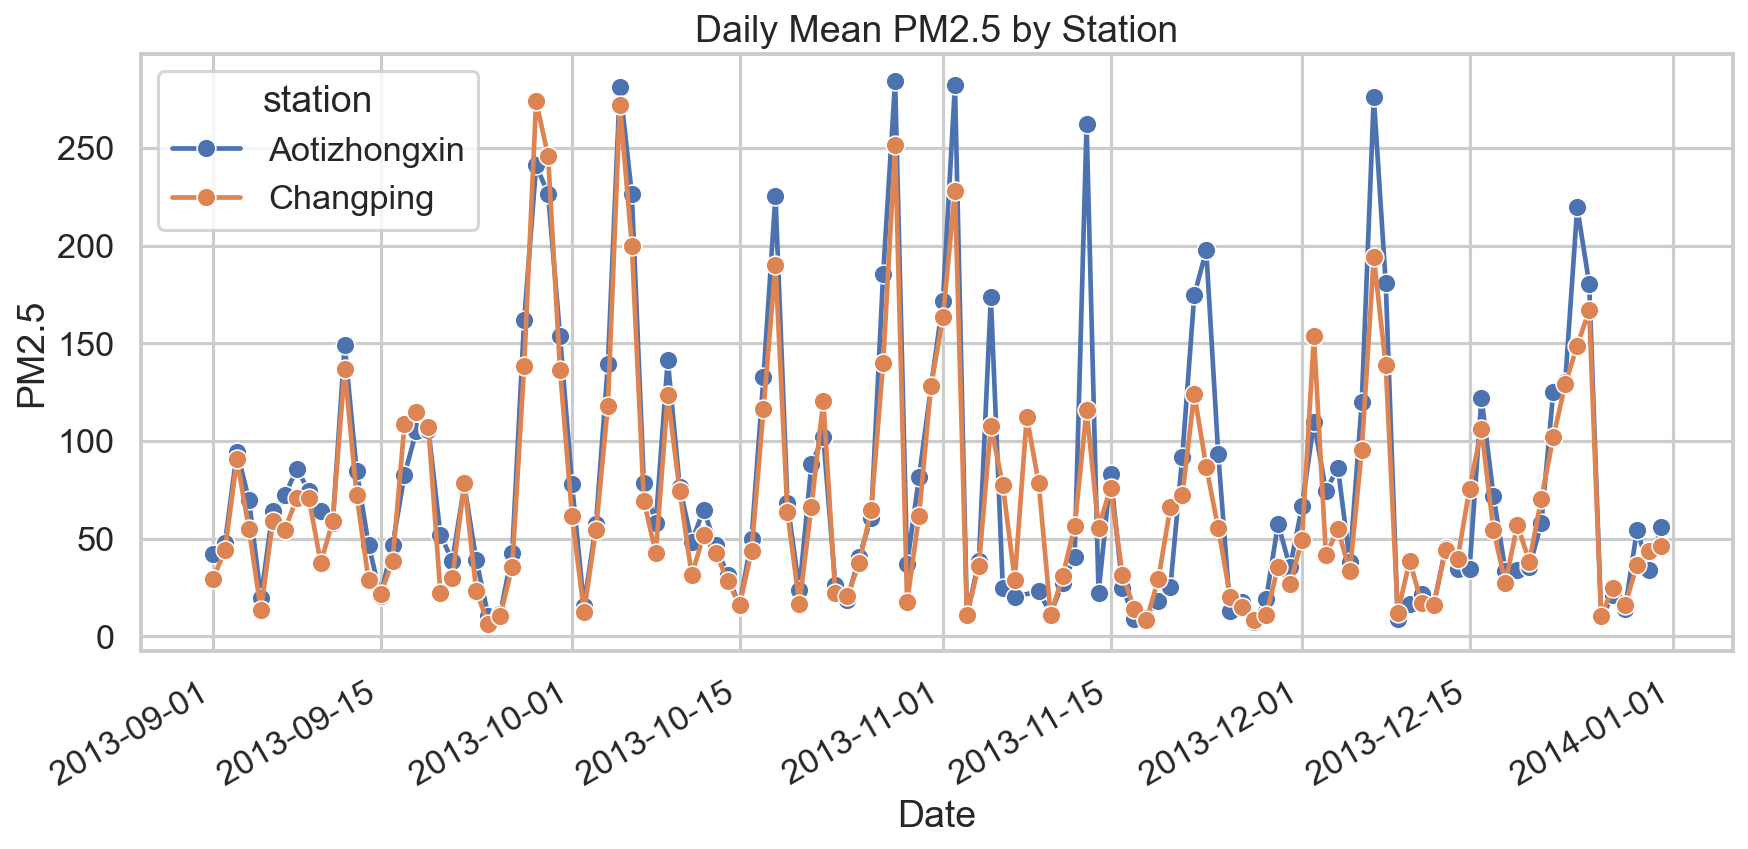
\includegraphics[width=0.78\textwidth]{pm25_timeseries.png}
\caption{Media giornaliera di \texttt{PM2.5} per stazione nel periodo analizzato.}
\end{figure}

\begin{figure}[H]
\centering
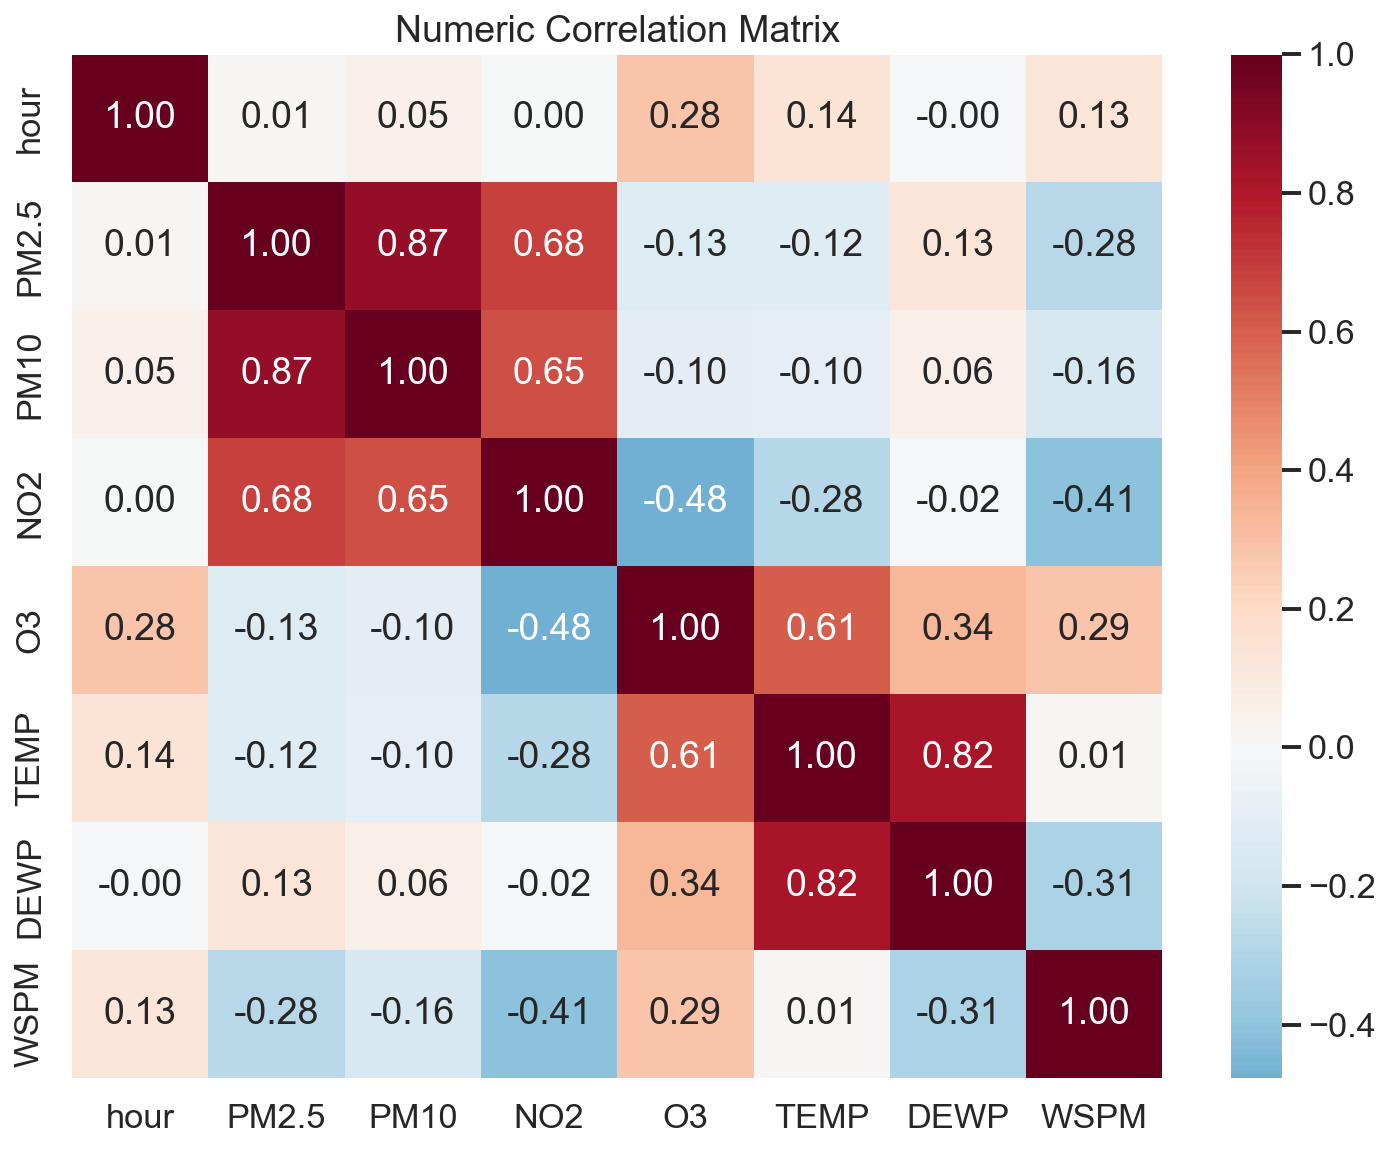
\includegraphics[width=0.78\textwidth]{correlation_matrix.png}
\caption{Matrice di correlazione delle variabili numeriche principali.}
\end{figure}

I risultati della validazione delle regole candidate in configurazione \texttt{medium} sono sintetizzati nella Tabella~\ref{tab:candidate}.

\begin{table}[H]
\centering
\caption{RFD candidate con soglie \texttt{medium}}
\label{tab:candidate}
\begin{tabularx}{\textwidth}{>{\raggedright\arraybackslash}X r r}
\toprule
Regola & Support & Confidence \\
\midrule
\texttt{station, PM2.5 $\rightarrow$ PM10} & 0.073 & 0.466 \\
\texttt{station, TEMP, WSPM $\rightarrow$ O3} & 0.035 & 0.385 \\
\texttt{hour, NO2 $\rightarrow$ PM2.5} & 0.026 & 0.317 \\
\texttt{station, hour, TEMP $\rightarrow$ NO2} & 0.009 & 0.254 \\
\texttt{station, TEMP, DEWP $\rightarrow$ PM2.5} & 0.014 & 0.203 \\
\bottomrule
\end{tabularx}
\end{table}

La regola pi\`u forte \`e \texttt{station, PM2.5 $\rightarrow$ PM10}. Il risultato \`e coerente con l'alta correlazione tra i due indicatori di particolato, ma la confidenza rimane modesta. In termini sostanziali, questo significa che osservazioni simili su \texttt{station} e \texttt{PM2.5} non conducono abbastanza spesso a valori simili di \texttt{PM10} da supportare una regola robusta.

Le altre regole candidate risultano ancora pi\`u deboli. In particolare, \texttt{station, TEMP, DEWP $\rightarrow$ PM2.5} ha una confidenza pari a 0.203, suggerendo che condizioni termo-igrometriche simili non bastano a spiegare un comportamento sufficientemente coerente del particolato fine. Allo stesso modo, \texttt{station, hour, TEMP $\rightarrow$ NO2} presenta supporto inferiore a 0.01 e quindi una copertura limitata del dominio osservato.

La variazione delle soglie conferma questo quadro. La regola \texttt{station, PM2.5 $\rightarrow$ PM10} passa da una confidenza di 0.374 in configurazione \texttt{strict} a 0.610 in configurazione \texttt{relaxed}; tutte le altre restano sotto tali valori. Nessuna raggiunge comunque la soglia finale di 0.85.

\begin{figure}[H]
\centering
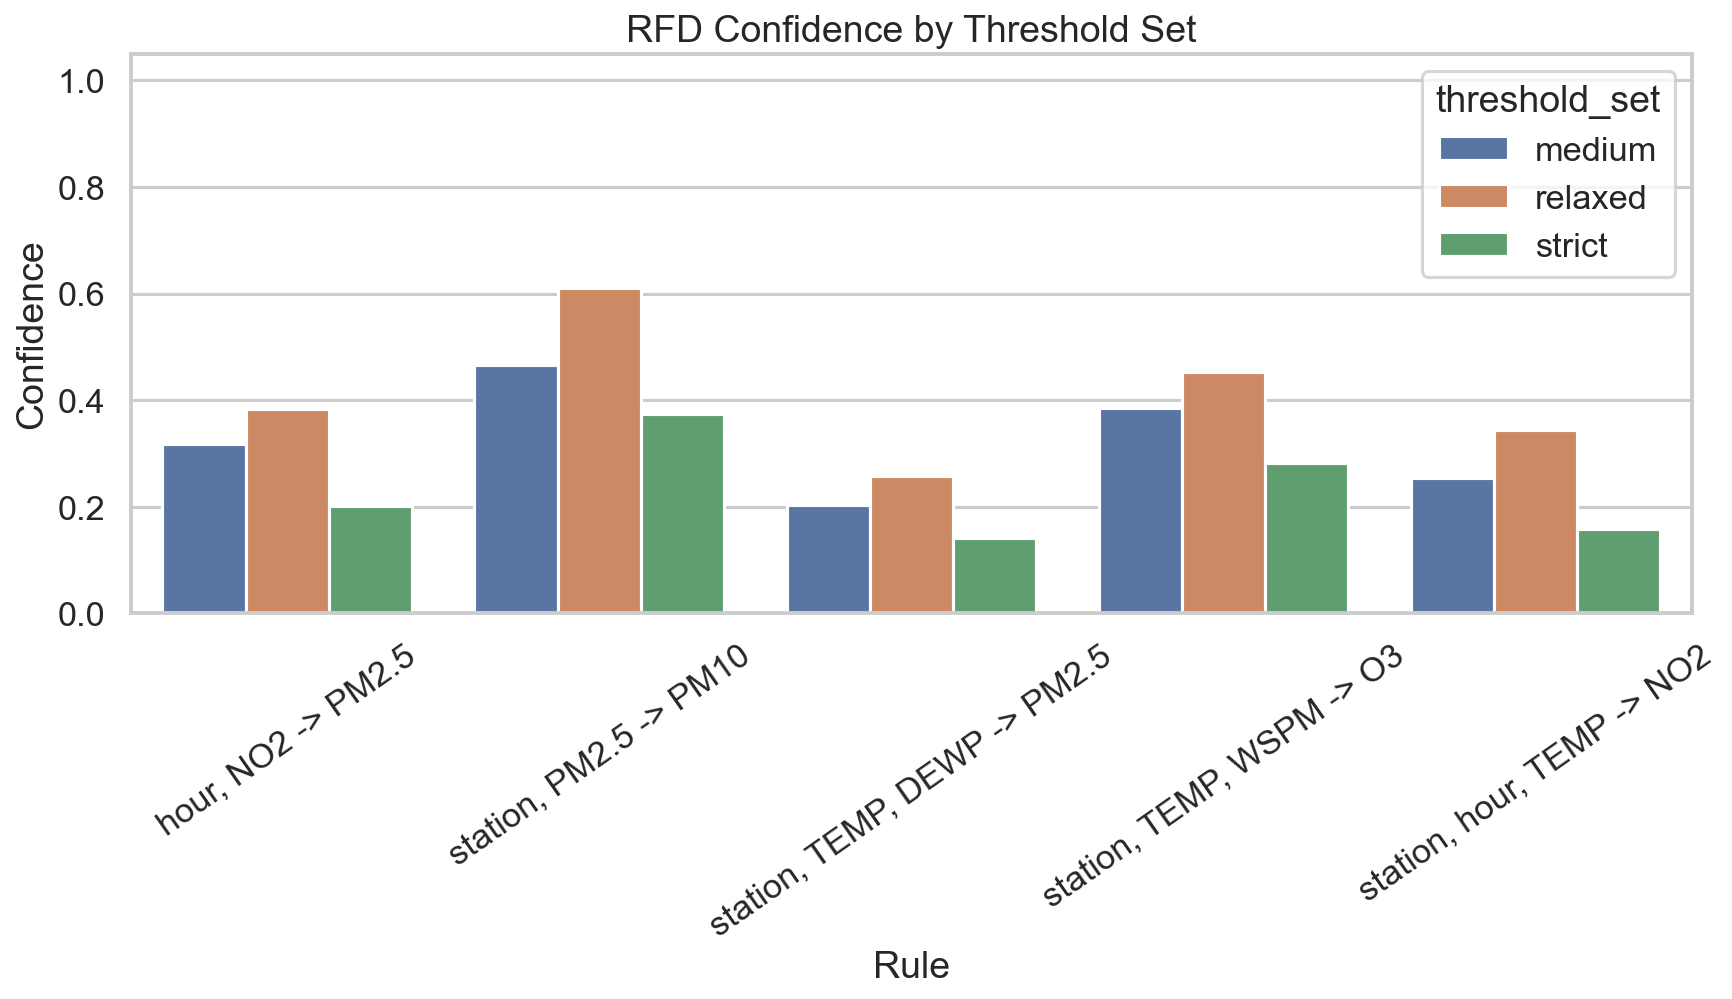
\includegraphics[width=0.82\textwidth]{rfd_confidence_by_threshold.png}
\caption{Confidenza delle regole candidate nelle tre configurazioni di soglia.}
\end{figure}

Per completezza, la Tabella~\ref{tab:thresholds-results} riassume l'andamento della confidenza nelle tre configurazioni.

\begin{table}[H]
\centering
\caption{Confronto delle confidenze al variare delle soglie}
\label{tab:thresholds-results}
\begin{tabular}{lccc}
\toprule
Regola & strict & medium & relaxed \\
\midrule
\texttt{station, PM2.5 $\rightarrow$ PM10} & 0.374 & 0.466 & 0.610 \\
\texttt{station, TEMP, WSPM $\rightarrow$ O3} & 0.283 & 0.385 & 0.452 \\
\texttt{hour, NO2 $\rightarrow$ PM2.5} & 0.201 & 0.317 & 0.383 \\
\texttt{station, hour, TEMP $\rightarrow$ NO2} & 0.159 & 0.254 & 0.345 \\
\texttt{station, TEMP, DEWP $\rightarrow$ PM2.5} & 0.142 & 0.203 & 0.258 \\
\bottomrule
\end{tabular}
\end{table}

La scoperta leggera non restituisce alcuna regola valida secondo i criteri finali. Il file \texttt{results/rfd\_discovered\_top10.csv} viene infatti esportato con la sola intestazione. Questo esito negativo \`e comunque rilevante: segnala che, nello spazio di ricerca definito, non emergono relazioni sufficientemente stabili da essere considerate RFD forti.

Il confronto per stazione mostra differenze moderate ma non risolutive. Ad esempio, \texttt{PM2.5 $\rightarrow$ PM10} ha confidenza 0.437 ad \texttt{Aotizhongxin} e 0.495 a \texttt{Changping}; \texttt{TEMP, WSPM $\rightarrow$ O3} \`e pi\`u forte ad \texttt{Aotizhongxin} (0.417) che a \texttt{Changping} (0.350). Anche l'analisi locale, dunque, non produce regole ad alta affidabilit\`a.

\begin{table}[H]
\centering
\caption{Confronto per stazione in configurazione \texttt{medium}}
\begin{tabular}{llcc}
\toprule
Regola valutata & Stazione & Support & Confidence \\
\midrule
\texttt{PM2.5 $\rightarrow$ PM10} & Aotizhongxin & 0.143 & 0.437 \\
\texttt{PM2.5 $\rightarrow$ PM10} & Changping & 0.151 & 0.495 \\
\texttt{TEMP, DEWP $\rightarrow$ PM2.5} & Aotizhongxin & 0.029 & 0.202 \\
\texttt{TEMP, DEWP $\rightarrow$ PM2.5} & Changping & 0.026 & 0.204 \\
\texttt{TEMP, WSPM $\rightarrow$ O3} & Aotizhongxin & 0.073 & 0.417 \\
\texttt{TEMP, WSPM $\rightarrow$ O3} & Changping & 0.066 & 0.350 \\
\texttt{hour, NO2 $\rightarrow$ PM2.5} & Aotizhongxin & 0.025 & 0.349 \\
\texttt{hour, NO2 $\rightarrow$ PM2.5} & Changping & 0.030 & 0.293 \\
\bottomrule
\end{tabular}
\end{table}

Un ulteriore elemento utile \`e l'analisi delle violazioni esportate. Per la regola \texttt{station, PM2.5 $\rightarrow$ PM10}, ad esempio, compaiono coppie di osservazioni nella stessa stazione con valori di \texttt{PM2.5} vicini ma differenze di \texttt{PM10} anche superiori a 50 unit\`a. Analogamente, per \texttt{station, TEMP, WSPM $\rightarrow$ O3} si osservano casi con temperatura e velocit\`a del vento comparabili ma con \texttt{O3} molto diverso. Questi esempi non vanno letti automaticamente come errori: possono riflettere eventi locali, variabili omesse o semplice irregolarit\`a del fenomeno.

\section{Discussione e conclusioni}
Il risultato complessivo \`e coerente con il dominio applicativo. La qualit\`a dell'aria urbana dipende da un insieme ampio di fattori atmosferici e antropici, molti dei quali non sono rappresentati nel dataset ridotto. In questo contesto, \`e plausibile che regole interpretabili basate su pochi attributi abbiano una capacit\`a descrittiva limitata.

Il contributo principale del lavoro non sta quindi nell'identificazione di dipendenze forti, ma nella costruzione di un workflow riproducibile di \textit{consistency profiling}. Le RFD si rivelano utili per:
\begin{itemize}[leftmargin=1.2cm]
    \item verificare la coerenza approssimata tra variabili ambientali;
    \item confrontare la stabilit\`a delle regole al variare delle soglie;
    \item evidenziare violazioni potenzialmente interessanti;
    \item mantenere un elevato livello di interpretabilit\`a.
\end{itemize}

Restano tuttavia chiari i limiti del lavoro: l'UDT \`e solo concettuale, la validazione pairwise \`e quadraticamente costosa, le soglie sono scelte manualmente e le RFD non devono essere lette come leggi causali. In sintesi, il progetto mostra che l'approccio \`e adatto a un'analisi esplorativa rigorosa e leggibile, ma non supporta conclusioni forti sulla dinamica causale della qualit\`a dell'aria.

Un possibile sviluppo futuro sarebbe estendere l'analisi a un numero maggiore di stazioni o introdurre strategie di campionamento e pruning pi\`u sofisticate per la scoperta delle RFD. Sarebbe inoltre utile confrontare soglie fissate manualmente con soglie derivate dai quantili empirici delle differenze tra osservazioni. Anche in questi casi, tuttavia, l'obiettivo resterebbe quello di descrivere regolarit\`a approssimate, non di stabilire nessi causali.

\begin{thebibliography}{9}

\bibitem{uci}
S. Chen.
\newblock \textit{Beijing Multi-Site Air Quality} [Dataset].
\newblock UCI Machine Learning Repository, 2017.
\newblock DOI: \url{https://doi.org/10.24432/C5RK5G}

\bibitem{rfd-survey}
L. Caruccio, V. Deufemia, and G. Polese.
\newblock Relaxed Functional Dependencies -- A Survey of Approaches.
\newblock \textit{IEEE Transactions on Knowledge and Data Engineering}, 28(1):147--165, 2016.

\bibitem{rfd-mining}
L. Caruccio, V. Deufemia, and G. Polese.
\newblock Mining relaxed functional dependencies from data.
\newblock \textit{Data Mining and Knowledge Discovery}, 34(2):443--477, 2020.

\end{thebibliography}

\end{document}
